\section{Esempi di funzionamento e limitazioni riscontrate}
\subsection{Test download}
\subsubsection{Output del test}

\textbf{PEER}
\begin{verbatim}
rating ram = 0.735992
rating cpu = 0.756667
CODICE PEER

JOIN (5) IP=160.80.146.107
comando ricevuto=ack
size=0
cont=5 RESULT=> ack
join effettuato a 160.80.146.107
----------------------------------

#COMANDI
1: LEAVE
2: UPDATE
3: WHOHAS
=>inserire il numero della scelta:
----------------------------------
3

quale file si vuole cercare?
roxanne.mp3

WHOHAS:roxanne.mp3 - cont=5
comando ricevuto=ack
size=4
ID=0
numero di ip 1
LISTA IP RESTITUITI
0 = 160.80.148.15

cont=5 RESULT OF THE OPERATION=> ack
esito della whohas di 'roxanne.mp3'  : 1
----------------------------------
#COMANDI
2: UPDATE
4: STOP (della ricerca)
=>inserire il numero della scelta:
----------------------------------
4

STOP (5)
comando ricevuto=ack
size=0
cont=5 RESULT=> ack
FINE RICERCA , ip trovati: 1
STAMPA LISTA
ELEM[0] IP= 160.80.148.15
digitare 1 se si vuole scaricare il file
1

AVVIO DEL DOWNLOAD DI roxanne.mp3 dal peer 160.80.148.15

INIZIO DOWNLOAD
nome file : roxanne.mp3
dimensione file: 4613617 
numero chunk file: 9010 
invio ack riuscito
-----------------
posizione in cui verrà salvato il file : Scaricati/roxanne.mp3
store
numero chunk già ricevuti di questo file: 0
file incompleto
**********
DOWNLOAD IN CORSO
**********
fine lettura da socket
transazione completata, file ricevuto senza errori
result inviato: ack

FINE DOWNLOAD
TEMPO IMPIEGATO PER IL DOWNLOAD = 12.035000
\end{verbatim}

\textbf{SUPERPEER}
\begin{verbatim}
comando ricevuto=join
size=108
ricevuto filtro
RATING:1.492659
STAMPA LISTA PEER
elem [0] ==> IP= 160.80.146.107, RAT= 1.492659

...

aggiornato TTL dell'IP 160.80.146.107 
comando ricevuto=whhs
size=11
ID=0
dati=roxanne.mp3
INIZIO CODICE WHOHAS
inserita la query
ricerca di : roxanne.mp3
lunghezza nome file:11
numero di peer connessi : 2
match del file roxanne.mp3 nel peer 160.80.148.15
IP trovati 1
ip 0 = 160.80.148.15 

result inviato

aggiornato TTL dell'IP 160.80.146.107 
comando ricevuto=stop
size=0
QUERY CANCELLATA DALLA LISTA
result inviato
...
\end{verbatim}
\subsubsection{Commento}
In questo test è mostrato come il peer entra nella rete (calcolando il suo rating iniziale e facendo la join a un superpeer), compie una ricerca e il successivo download del file cercato.\linebreak
Come si può vedere all'utente è fornito un menù testuale nel quale vengono fornite delle voci selezionabili inserendo da tastiera il numero relativo alla scelta.\linebreak
Nel caso di una ricerca, dopo aver selezionato la giusta scelta nel menu, il programma chiede anche il nome del file che si vuole scaricare inviando un messaggio di whohas al suo superpeer specificando il file cercato.\linebreak 
Il superpeer risponderà con i dati relativi ai peer a lui connessi e restituendo la lista dei peer che hanno il file.\linebreak
\begin{verbatim}
numero di ip 1
LISTA IP RESTITUITI
0 = 160.80.148.15
\end{verbatim}
A questo punto il peer rimane in attesa di altri risultati successivi fino a che l'utente non specifica uno stop (che nel frattempo è apparso nel menù di scelta). Una volta che l'utente ha bloccato la ricerca il peer inizia la fase di download, che nell'output sopra è compreso tra la stampa "INIZIO DOWNLOAD" e "FINE DOWNLOAD".\linebreak
In questo esempio il file non era presente (neanche in parte) sul peer, e quindi è stato scaricato dal chunk 0. Se il file fosse già stato parzialmente ricevuto si avrebbe avuto una stampa del tipo: \textit{numero chunk già ricevuti di questo file: 135}; e il download sarebbe stato eseguito esattamente uguale solo partendo da tale chunk.\linebreak
Nell'esecuzione del superpeer si può vedere come esso ricevi e processi i comandi inviati dal peer. Quando riceve una whohas inserisce la query in una lista con i riferimenti delle ricerche in corso, effettua il controllo sui peer a lui connessi e risponde al peer.

\subsection{Test switch peer-superpeer}
\subsubsection{output del test}
\textbf{SUPERPEER}
\begin{verbatim}

ENTRATO IN ISSET UDP
aggiornato TTL dell'IP 160.80.146.107 
comando ricevuto=ping
size=8
aggiornato rating (1.493180) dell'IP 160.80.146.107 

INIZIO OPERAZIONE SWITCH
inviato messaggio di pong al peer
inviato leave al bootstrap
invio messaggio di leave dal SP a 160.80.148.15
FINE SUPERPEER

\end{verbatim}
\textbf{PEER}
\begin{verbatim}
[...]

PEER:	
ricevuto nwsp da: 160.80.148.15
comando ricevuto=nwsp
size=1

SUPERPEER:
register=1

ENTRATO IN ISSET UDP
comando ricevuto=join
size=108
ricevuto filtro
RATING:0.686023

STAMPA LISTA PEER
elem [0] IP= 160.80.148.15, RAT= 0.686023
result inviato


ENTRATO IN ISSET UDP
comando ricevuto=join
size=108
ricevuto filtro
RATING:1.493180

STAMPA LISTA PEER
elem [0] IP= 160.80.146.107, RAT= 1.493180
elem [1] IP= 160.80.148.15, RAT= 0.686023

result inviato

\end{verbatim}

\subsubsection{Commento}
Il superpeer che riceve il ping da un peer con rating sufficentemente maggiore del suo, avvia l'operazione di switch. Quindi abbandona la rete come superpeer effettuando la leave al bootstrap e informa i peer (escluso quello che ha pingato) a lui connessi che sta abbandonando la rete informandoli dell'ip del nuovo superpeer, in questo caso solo 160.80.148.15.\linebreak
Il peer che deve deve diventare superpeer riceve il comando di "nwsp" e avvia il processo del superpeer, al quale si connetteranno i peer che erano connessi al superpeer che ha abbandonato la rete (160.80.146.107, 160.80.148.15).


\subsection{Test ricerca}
\subsubsection{output del test}
\begin{verbatim}
ENTRATO IN ISSET UDP
aggiornato TTL dell'IP 160.80.146.107 
comando ricevuto=whhs
size=7
ID=0
dati=gdl.pdf

INIZIO CODICE WHOHAS
inserita la query
inoltro sulla rete di overlay
ricerca di : gdl.pdf
lunghezza nome file:7
numero di peer connessi : 1
IP trovati 0
result inviato

[...]

NUMERO SUPERPEER CONNESSI : 1
ENTRATO IN ISSET TCP
comando ricevuto=ack
size=5
ID=1
dati=;ipvicini
aggiungere nella try list: 160.80.128.69
INOLTRO WHOHAS
FINE ISSET TCP

[...]

ENTRATO IN ISSET UDP
comando ricevuto=ack
size= 9
ID= 1
dati= ippeer;ipvicini

[...]

ENTRATO IN ISSET UDP
aggiornato TTL dell'IP 160.80.146.107 
comando ricevuto=stop
size=0
QUERY CANCELLATA DALLA LISTA
result inviato

\end{verbatim}

\subsubsection{commento}
In questo test viene illustrato il caso in cui una ricerca viene inoltrata sulla rete d'overlay passando sia sulle connesioni TCP che UDP. Il messaggio di whohas viene quindi mandato al superpeer di riferimento del peer, il quale controlla la presenza del file sui propri peer, memorizza la query associata alla ricerca ed inoltra la ricerca sui suoi vicini con cui comunica in TCP.
\begin{verbatim}
INIZIO CODICE WHOHAS
inserita la query
inoltro sulla rete di overlay
ricerca di : gdl.pdf
lunghezza nome file:7
numero di peer connessi : 1
IP trovati 0
result inviato
\end{verbatim}
Il superpeer dopo aver inoltrato la richiesta riceve le risposte dai vicini che conterranno gli ip in cui è stato matchato il file e gli ip dei vicini del superpeer che ha inviato la risposta. Gli indirizzi dei peer che hanno il file verranno inoltrati al peer che ha effettuato la ricerca mentre gli indirizzi dei superpeer verranno aggiunti alla try-list e successivamente contattati in udp e memorizzati in done-list.\linebreak
I vicini dei vicini che ricevono la whohas risponderanno sempre indicando i peer che hanno il file e i superpeer vicini.
\begin{verbatim}
ENTRATO IN ISSET UDP
comando ricevuto=ack
size= 9
ID= 1
dati= ippeer;ipvicini
\end{verbatim}
Queste operazioni continuano finchè non viene ricevuto il comando di stop dal peer o viene raggiunto il numero massimo di peer o superpeer contattati.

\subsection{Limitazioni riscontrate}
Una delle principali limitazioni riscontrate è che, usando i filtri di bloom per memorizzare le informazioni sui file dei peer, non è possibile cercare un file di cui non si conosca il nome esatto con la propria estensione. Inoltre il superpeer non sà esattamente quali file sono presenti nei peer connessi, però può interrogare i filtri associati ad ogni peer, in modo tale da sapere se il file cercato è presente o no. \linebreak
Un altro problema nell'uso dei filtri di bloom è quello dei cosiddetti "falsi positivi", ossia che l'interrogazione del filtro potrebbe avere esito positivo nonostante il file non sia presente.
Questo problema però è meno importante del primo, in quanto la probabilità di errore risulta essere trascurabile (minore del 10\%) finchè gli elementi condivisi sono meno di 900 circa (come si puo vedere in figura \ref{falsi}).

\begin{figure}[h]
\centering
{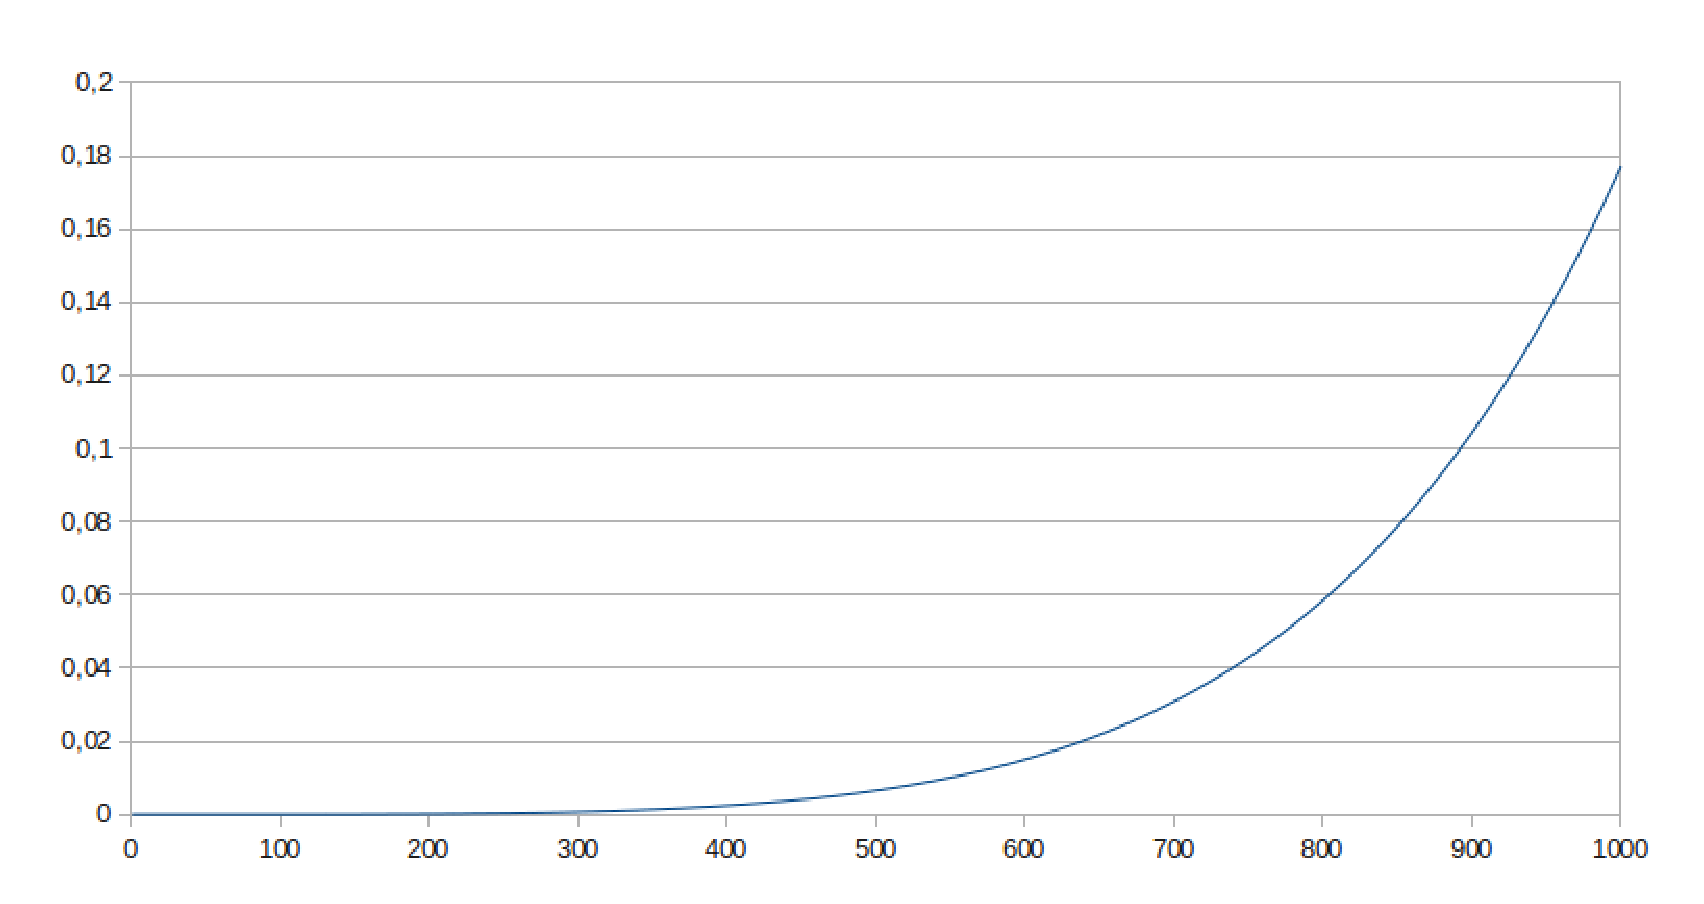
\includegraphics[width=10cm]{img/falsi}}
\caption{Probabilità di falsi positivi al variare del numero degli elementi condivisi\label{falsi}}
\end{figure}

Nonostante è problematico cercare file di cui non si conosca il nome esatto, l'uso dei filtri di bloom garantisce efficenza e scarsa occupazione in memoria. Inoltre, utilizzando un numero di funzioni hash maggiore la probabilità di falsi positivi diminuirebbe ulteriormente.\linebreak

Un ulteriore limitazione è che non è possibile per un peer svolgere ricerche e download in parallelo, in quanto sono state implementate come operazioni seriali. Ovviamente i superpeer possono gestire più ricerche in parallelo come specificato nel capitolo relativo alla fase di lookup.\linebreak

Non è possibile contattare computer dietro a NAT o firewall in quanto non sono raggiungibili a meno di un settaggio specifico di router e firewall.\linebreak

Nonostante il sistema sia parzialmente distribuito, in caso di caduta del server di bootstrap, è impossibile per nuovi peer l'entrata nella rete, anche se quest'ultima potrebbe continuare a svolgere il suo lavoro normalmente.\linebreak

